\pagestyle{empty}
\centering
\fontsize{2cm}{2cm}\selectfont{Module Design Document} \\
\vspace{2mm}
\fontsize{1cm}{1cm}\selectfont Audio digital signal processor \\
\vspace{2mm}
\large BeCreative Minor\\
\normalsize
\vspace{4cm}
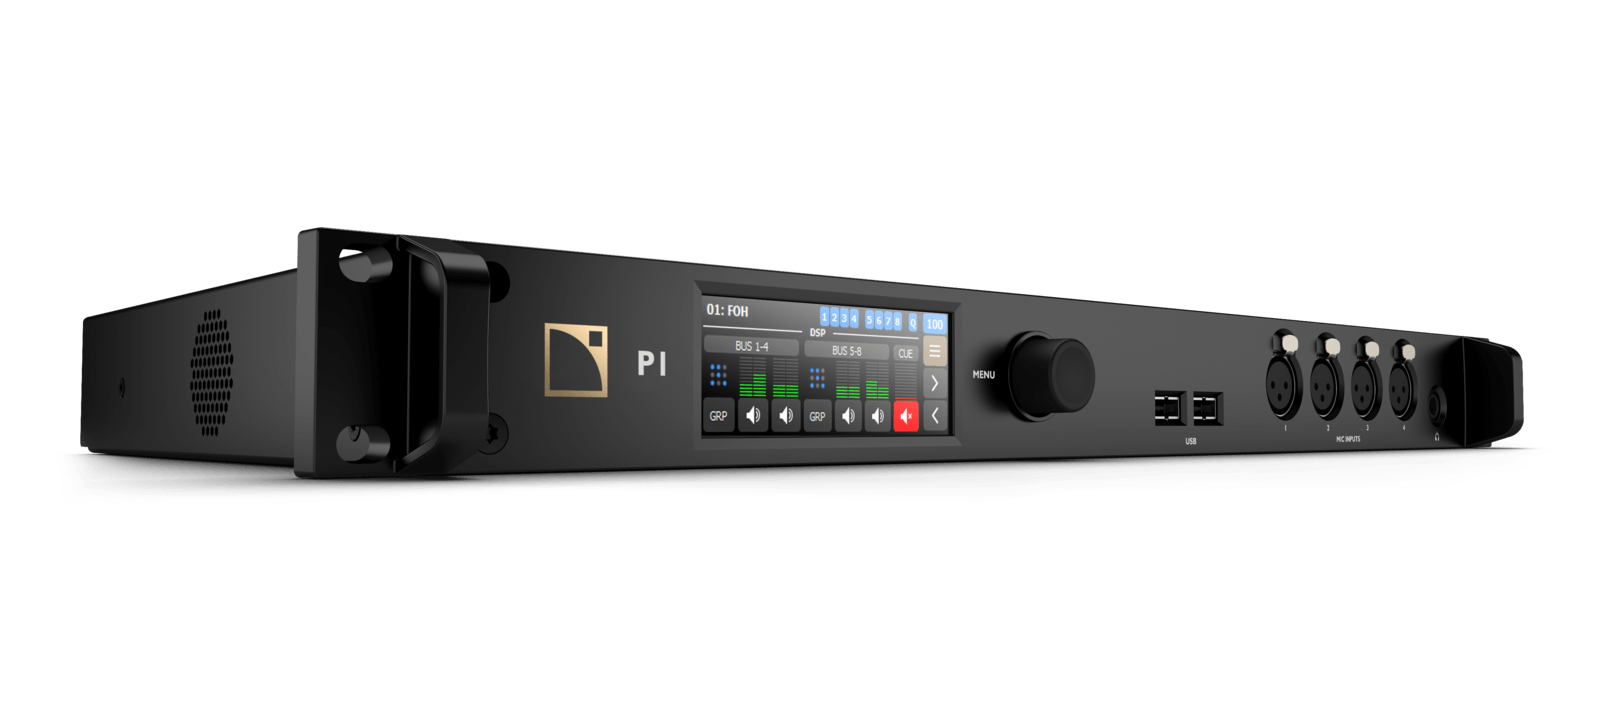
\includegraphics[width=\linewidth]{3DR_P1_Perspective.png}\\
\vfill
\normalsize Busse Lommers \\
Robin van den Dungen \\
Mahmud Gürler \\
Silas Kamphuis \\
Hein Verhallen \\
Youri Tils \\
Fontys Hogescholen, De Rondom 1, 5612 AP Eindhoven \\
\today

\begin{justify}

\chapter*{Summary}
The following text translates to English as:

This report describes how this project group created an audio DSP for the BeCreative Minor. This was done because the members of the group wanted to learn more about it and improve their technical knowledge.

Chapter "Problem Description" outlines the project's background and goals. Chapter "Research" describes the preliminary investigations conducted. Chapter "Concept Development" explains how the product concept was developed. Chapter "Realization" details the actual design of the audio DSP. Chapter "Verification" discusses the product testing process. Finally, in chapters "Conclusions" and "Recommendations," the conclusion and recommendations are respectively described.

\newpage
\tableofcontents
\thispagestyle{empty}

\listoffigures
\thispagestyle{empty}

\listoftables
\thispagestyle{empty}

\newpage
\pagestyle{plain}

\chapter*{Report contribution}	%Fill-in only regarding the report contribution.
\begin{longtable}{|c|c|c|}
	\hline
	\textbf{Chapter} & \textbf{Paragraph} & \textbf{Person} \\ \hline
	Problem Description			& Background					& All	 					\\ \hline
	Introduction				& NA							& Busse 					\\ \hline
								& Problem description			& Robin						\\ \hline
								& Project goals					& All						\\ \hline
								& Requirements					& All 						\\ \hline
								& Project scope					& All 						\\ \hline
								& Boundary condition			& All						\\ \hline
								& Project approach				& All						\\ \hline
								& Verification method			& All						\\ \hline
	Research 					& Research objectives			& All 						\\ \hline
								& Research questions			& All 						\\ \hline
								& Research approach				& All 						\\ \hline
								& Results						& All 						\\ \hline
	Concept Development 		& Concept overview				& Youri						\\ \hline
								& Front-end						& Silas						\\ \hline
								& Audio-DSP						& Youri						\\ \hline
								& Back-end						& Silas						\\ \hline
								& Interfacing					& Robin						\\ \hline
								& Front-end						& Robin						\\ \hline
								& Audio-DSP						& Youri						\\ \hline
								& Back-end						& Robin						\\ \hline
								& Power supplies				& Mahmud \& Robin			\\ \hline
								& Modules						& Busse						\\ \hline
								& UI							& Hein \& Busse				\\ \hline
								& Hardware programming			& Busse						\\ \hline
								& Hardware design				& Busse						\\ \hline
								& Design decissions				& Busse						\\ \hline
	Realization					& Hardware						& NA						\\ \hline
								& Schematic						& Robin						\\ \hline
								& Printed circuit board			& Silas						\\ \hline
								& Case							& Busse						\\ \hline
								& Firmware						& Youri						\\ \hline
								& I2S decoder and encoder		& Youri						\\ \hline
								& I2C controller				& Youri						\\ \hline
								& Band-pass filter				& Youri						\\ \hline
								& Sinewave generator			& Youri						\\ \hline
								& Effects						& Youri \& Busse			\\ \hline
								& User interface				& Hein \& Busse				\\ \hline
								& User interface				& Hein \& Busse				\\ \hline
	Verification				& Method						& Robin						\\ \hline
								& Hardware						& Mahmud \& Robin			\\ \hline
								& Firmware						& Youri						\\ \hline
								& Results						& NA						\\ \hline
								& Hardware						& Mahmud					\\ \hline
								& Firmware						& Youri						\\ \hline
								& Conclusions					& Mahmud \& Silas \& Robin 	\\ \hline
								& Hardware						& Mahmud					\\ \hline
								& Firmware						& Youri						\\ \hline
	Conclusions					& NA							& Silas						\\ \hline
	Recommendations				& NA							& Silas						\\ \hline
	Summary						& NA							& Robin						\\ \hline
	Bibliography				& NA							& Busse						\\ \hline
	Appendix A: State-space		& NA							& Youri						\\ \hline
	Appendix B: VHDL code		& I2S decoder					& Youri						\\ \hline
								& I2S encoder					& Youri						\\ \hline
								& I2C master					& Youri						\\ \hline
								& State-space BPF code			& Youri						\\ \hline
								& Sinewave generator code		& Youri						\\ \hline
	Appendix C: Schematics		& Buck converter schematic		& Mahmud					\\ \hline
								& SEPIC schematic				& Silas						\\ \hline
								& Linear regulator schematic	& Silas	\& Robin			\\ \hline
								& Main board schematic			& Robin						\\ \hline
								& Buck converter calculations	& Silas						\\ \hline
								& SEPIC calculations			& Robin						\\ \hline
	Appendix D: UI design		& Main menu						& Busse						\\ \hline
								& Adjust preset menu			& Busse						\\ \hline
	Appendix E: Case			& Top view						& Busse						\\ \hline
								& Front view					& Busse						\\ \hline
								& Rear view						& Busse						\\ \hline
	Appendix F: Verification	& Ground spring					& Robin						\\ \hline

	\caption{Revision list of the document}
	\label{table:revision_history}
\end{longtable}

\newpage
\pagestyle{plain}
\setcounter{page}{1}

\chapter*{Abbreviation List}

\begin{table}[!h]
	\centering
	\begin{tabular}{|c|c|}
		\hline
		\textbf{Abbreviation} & \textbf{Explanation}	\\ \hline
		DSP 					& Digital Signal Processor    				\\ \hline
		ADC 					& Analog-to-Digital Converter 				\\ \hline
		BPF 					& Band-Pass Filter							\\ \hline
		CH 						& Channel									\\ \hline
		DAC 					& Digital-to-Analog Converter 				\\ \hline
		FFT 					& Fast Fourier Transform					\\ \hline
		FPGA 					& Field programmable gate array 			\\ \hline
		GBW 					& Gain Bandwidth Product 					\\ \hline
		RAM 					& Random Access Memory	    				\\ \hline
		SEPIC        			& Single-Ended Primary-Inductor Converter	\\ \hline
		SINAD 					& Signal to noise and distortion 			\\ \hline
		TRS 					& Tip ring sleeve connector (jack) 			\\ \hline
	\end{tabular}
	\caption{List of commonly used Abbreviations}
	\label{table:Abbreviation list}
\end{table}